\documentclass[english,hidelinks,pdftex, 11 pt, class=report,crop=false]{standalone}
\usepackage[T1]{fontenc}
\usepackage[utf8]{luainputenc}
\usepackage{geometry}
\geometry{verbose,paperwidth=16.4 cm, paperheight=29cm, inner=2.05cm, outer=2.05 cm, bmargin=2cm, tmargin=1.8cm}
\usepackage{import}
\usepackage[subpreambles=false]{standalone}
\usepackage{amsmath}
\usepackage{amssymb}
\usepackage{esint}
\usepackage{babel}
\usepackage{tabu}
\setlength{\parindent}{0bp}
\usepackage{enumitem}
\usepackage{xcolor}

\begin{document}
\huge \textbf{Lekser i matematikk veke 44}\\
\normalsize Leverast innnan torsdag
 \\[25pt]
\large
{\Large \textbf{Oppgåve 1}}\\[10pt]
\textit{Eksempel:}
\begin{figure}
	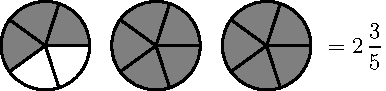
\includegraphics[]{bra}
\end{figure}
a) \\
\includegraphics[]{brb} \\
b) \\
\includegraphics[]{brc}
c) \\
\includegraphics[]{brd}
\\[25pt]
{\Large \textbf{Oppgåve 2}}\\[10pt]
Gjer om til uekte brøk.\\[5pt]
\textit{Eksempel:} $ \displaystyle {\color{blue}3}\,\frac{2}{\color{orange}5}=\frac{{\color{blue}3}\cdot{\color{orange}5}+2}{\color{orange}5}=\frac{15+2}{5}=\frac{17}{5} $
\begin{enumerate}[label=\alph*)]
	\item $ 4\,\dfrac{3}{7} $ \\[5pt]
	\item $ 8\,\dfrac{2}{9} $ \\[5pt]
	\item $ 10\,\dfrac{1}{6} $ \\[5pt]	
	
	
\end{enumerate}


\newpage	
\footnotesize OBS! Hugs å skrive namn på arket \\[25pt]
\large

{\Large \textbf{Oppgåve 3}}\\[10pt]
Vis utrekning slik som i eksempelet. \\[10pt]
\textit{Eksempel:} $ \displaystyle
\frac{2}{\color{blue}9}+\frac{3}{\color{orange}4}=\frac{2\cdot \color{orange}4}{9\cdot\color{orange}4}+\frac{3\cdot\color{blue}9}{4\cdot\color{blue}9}=\frac{8}{36}+\frac{27}{36}=\frac{35}{36}$ \\[10pt]
\begin{enumerate}[label=\alph*)]
	\item $\displaystyle \dfrac{2}{3}+\frac{5}{7} $\\[15pt]
	\item $\displaystyle \dfrac{3}{2}+\frac{8}{9}$\\[15pt]
	\item $\displaystyle \dfrac{9}{6}+\frac{1}{4} $\\[15pt]
	\item $\displaystyle \dfrac{7}{5}-\frac{3}{8} $\\[15pt]	
	\item $\displaystyle \dfrac{9}{4}-\frac{2}{3} $\\[15pt]
	\item $\displaystyle \frac{7}{2}-\dfrac{12}{5} $\\[15pt]	
	\item $\displaystyle \frac{10}{3}-\dfrac{21}{10} $\\[15pt]		
\end{enumerate}




\end{document}

